\documentclass[a4paper,11pt]{report}
\usepackage{style}
\makeglossaries
\newacronym{ac}{AC}{alternating current}
\newacronym{aps}{APS}{active pixel sensor}
\newacronym{ccd}{CCD}{charge-coupled device}
\newacronym{cdc}{CDC}{clock domain crossing}
\newacronym{cfa}{CFA}{colour filter array}
\newacronym{cmos}{CMOS}{complementary metal-oxide-semiconductor}
\newacronym{csi}{CSI}{camera serial interface}
\newacronym{dci}{DCI}{Digital Cinema Initiatives}
\newacronym{dslr}{DSLR}{digital single-lens reflex}
\newacronym{dut}{DUT}{design under test}
\newacronym{fpga}{FPGA}{field-programmable gate array}
\newacronym{fps}{FPS}{frames per second}
\newacronym{hdl}{HDL}{hardware description language}
\newacronym{hdmi}{HDMI}{High-Definition Multimedia Interface}
\newacronym{io}{IO}{input / output}
\newacronym{mipi}{MIPI}{Mobile Industry Processor Interface}
\newacronym{pcb}{PCB}{printed circuit board}
\newacronym{qvga}{QVGA}{quarter VGA}
\newacronym{ram}{RAM}{random-access memory}
\newacronym{sccb}{SCCB}{serial camera control bus}
\newacronym{soc}{SoC}{system-on-chip}
\newacronym{usb}{USB}{universal serial bus}
\newacronym{vga}{VGA}{video graphics array}

\title{Design of a Standardised Interface for Image Sensors}
\author{Michael Wild -- m.a.wild@se12.qmul.ac.uk \and Supervisor: Miles Hansard -- miles.hansard@qmul.ac.uk}
\date{\today}

\begin{document}
  \maketitle
  \begin{abstract}
Don't forget to fill this!!!!!
\end{abstract}

\renewcommand{\abstractname}{Acknowledgements}
\begin{abstract}
I would like to extend my thanks to Miles Hansard for giving me the freedom to propose and pursue my own project.
\end{abstract}

  \tableofcontents
  \listoffigures
  \listoftables
  \lstlistoflistings

  \chapter{Introduction}

Modern cameras -- both still-motion and video -- feature a high level of upgradability: lenses, filters and other accessories are all interchangeable, permitting finer control. As one of the most important components of the system, the image sensor plays a vital role in the composure of the final image. It dictates not only the output resolution, but also light sensitivity, colour representation, frame-rate and crop-factor. In spite of its significance, only a handful of expensive cinema and medium-format cameras include interchangeable sensors; even then, these components are proprietary. Upgrading the sensor in a mainstream camera requires the purchase of an entirely new system.

This paper details an FPGA-based sensor-agnostic interface which can be used to connect any image sensor to any image processor, thus providing the basis for a truly modular and upgradable camera system.

\section{A brief history of camera technology}

Modern cameras can trace their humble beginnings back to the camera obscura first described by ancient Chinese philosopher Mozi, who discovered an optical trick to pass light from an external scene through a hole and project it on a surface \cite{1_woolfson_2012}. In around 1816, French inventor Nicéphore Niépce managed to capture the first camera images using paper treated with silver chloride \cite{2_stokstad_cateforis_addiss_2005}. Continuing his work, Niépce's partner Louis Daguerre developed the first conventional camera using a simple lens to focus light onto a silver-coated copper plate \cite{3_harvard_library_preservation}.

\begin{figure}
  \centering
  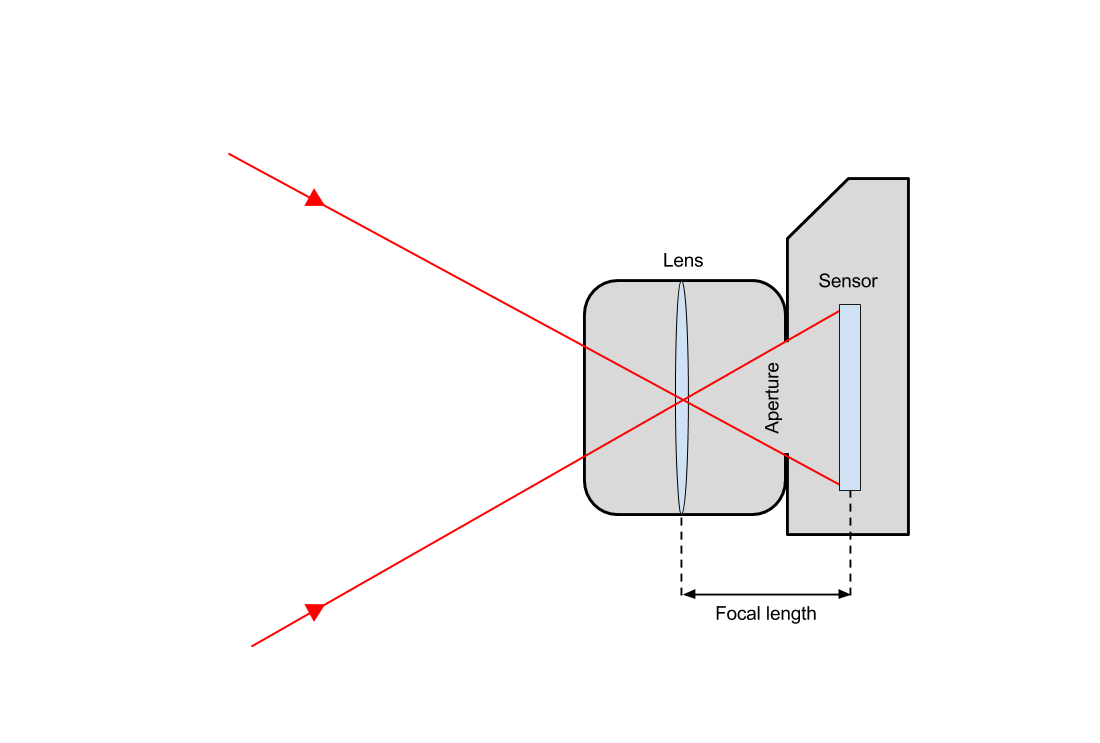
\includegraphics[width=1\textwidth]{./img/camera_physics_diagram.png}
  \caption{Light entering a camera and hitting sensor element}
  \label{fig:camera_physics_diagram}
\end{figure}

Figure \ref{fig:camera_physics_diagram} illustrates a very basic camera. Light from an external scene is focused by a lens and passed through an aperture hole where it is projected, inverted, onto a photosensitive surface for capture. The focal length dictates the distance between the optical centre of the lens and the sensor when the lens is focused to infinity \cite{4_pot_2010}. A shutter mechanism behind the aperture is used to control how much light hits the surface of the sensor, thus exposing the image. There are multiple ways to increase image exposure: expanding the aperture, holding the shutter open for longer, or increasing the ISO sensitivity of the sensor. Inversely, narrower apertures, shorter exposure times and lower sensitivities all decease the amount of light that hits the sensor, resulting in a darker image. 

Following the invention of the first transistor at Bell Laboratories in 1947, electronic devices could be dramatically reduced in size through the use of integrated circuits, paving the way for the start of the digital era \cite{5_computer_history_museum}. The first self-contained digital camera was developed by Steve Sasson of Eastman Kodak in 1975. Instead of using film, Sasson focused the light onto a state-of-the-art digital image sensor based on the first \gls{ccd} invented by Bell Laboratories scientists Willard Boyce and George Smith), the output of which was saved to a tape cassette for later viewing on a TV \cite{6_information_for_the_public,7_sasson_2007}.

Today, there are many different camera formats available -- one of the key differentiators being the area of the image sensor. A larger sensor can capture more light and thus the dynamic range is greatly increased, resulting in higher image quality \cite{8_chen_catrysse_el_gamal_wandell_2000}. This is true of both digital sensors, and their film counterparts.

\section{Motivation}

Professional camera systems are second-to-none when it comes to image quality and usability. The camera accessories market in Western Europe and the USA was worth \$1.7bn in 2006, a market which owed its existence to the modularity of modern cameras. With \$270 of accessories bought per \gls{dslr} camera on average, customisability is clearly an important feature \cite{9_understanding_and_solutions_2007}. Despite this, cameras lack customisability in one key area: IO expansion. Audio, video and storage interfaces are usually a fixed function of the camera's motherboard, and therefore non-interchangeable -- users must pre-empt their requirements in order to 'futureproof' their purchase. Inevitably these performance limits will be met; if a user wishes to step beyond these limits then an entirely new camera must be purchased. While some parts will undoubtedly be at the cutting edge of technology and require semi-frequent upgrades, other parts (camera bodies, audio amplifiers) may be technologically more mature and adhere to longer progression time-scales; thus it seems wasteful and costly to re-purchase these parts when buying a new camera system.

It is not the intent of this paper however, to suggest that the concept of an interchangeable camera sensor is entirely original -- a few high-end medium / large format cameras -- designed by Hasselblad, Phase One and Mayima -- exist which support interchangeable 'sensor backs' , however the interfaces are proprietary, thus limiting the user to a small handful of first-party options. Additionally, the prohibitively high price (upwards of \$10,000 at the time of writing) puts them far out of reach for the average professional photographer. Rather, the motivation of this project is to design an open standard for interchangeable sensors which can be freely implemented by anyone. In doing so, the basis for a truly modular and upgradable camera system is provided, with a broad range of applications including cinema, photography and computer vision. Figure \ref{fig:sensor_module} illustrates how this might work in practice. While idealistic, an open standard would benefit consumers by enabling new companies to gain a foothold serving smaller, more specialised markets which are too niche for established companies such as Nikon and Canon. Ultimately, this project aims to improve the camera selection available to consumers in the future by improving expandability options and fostering openness.

\begin{figure}
  \centering
  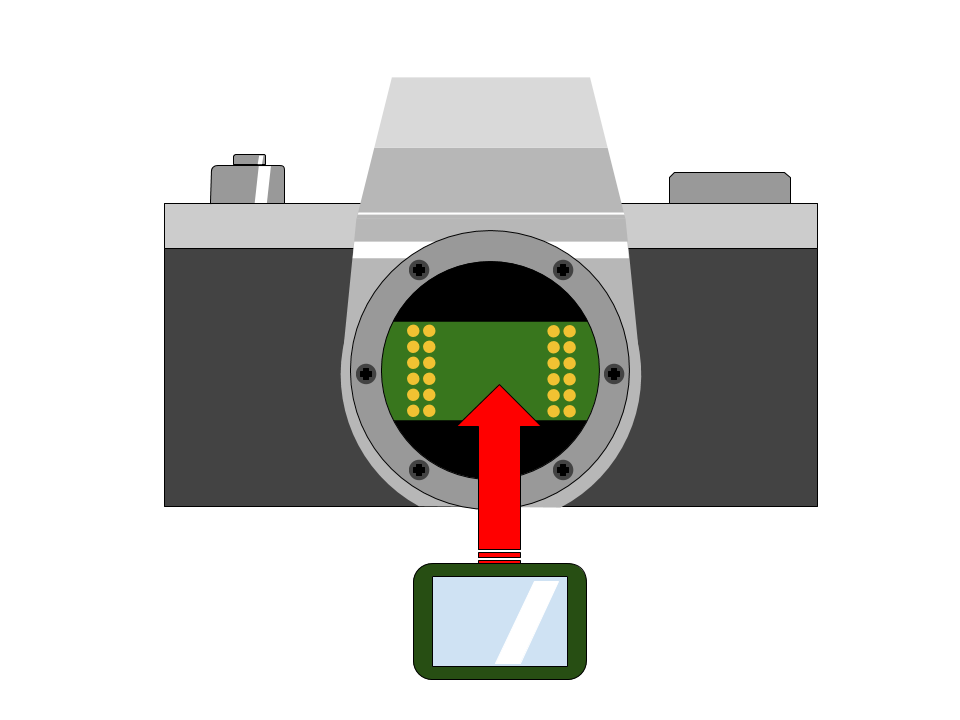
\includegraphics[width=1\textwidth]{./img/sensor_module.png}
  \caption{Inserting the sensor module into a camera}
  \label{fig:sensor_module}
\end{figure}



\section{Project testing platform}

The design of a full camera system is beyond the scope of this project, however an image sensor produced by OmniVision is used to capture real-world image data, providing a realistic test environment. \Glspl{fpga} are used extensively to set up a reconfigurable interface between the sensor and processor sides of the link, as well as generate test patterns for synthetic throughput and reliability tests. Given the main requirement of a sensor-agnostic interface is to work with a large range of sensors, there is a heavy emphasis on evaluating the system performance across several key metrics:

\begin{itemize}
  \item Reliability -- preserving signal integrity and ensuring low bit error rates for a stable and trustworthy system.
  \item Scalability -- transferring data across a wide range of resolutions and framerates to maintain a high level of expandability.
  \item Maximum throughput -- ensuring that the sensor interface does not bottleneck the system.
\end{itemize}

\subsection{Introduction to test system architecture}

The test system detailed in Figure \ref{fig:block_diagram_overview} is mainly based around the Zynq \gls{fpga} platform from Xilinx -- a programmable \gls{soc} with an embedded ARM core. \Glspl{fpga} are used instead of microcontrollers for several reasons, primarily because of the far greater flexibility of programmable logic, but also due to the high number of \gls{io} pins and throughput capabilities required to interface with high-resolution image sensors. \Glspl{fpga} are massively parallel and contain reconfigurable logic as well as multi-gigabit transceivers. Microcontrollers on the other hand, rely on fixed peripherals for a limited range of interface support; those which are not supported by the built-in peripherals must utilise bit-banging -- the process of using software to control the timing, synchronisation and state of \gls{io} ports to transmit or receive data. Microcontrollers simply lack the horsepower and resources to bit-bang a custom high-speed serial interface.

\begin{figure}
  \centering
  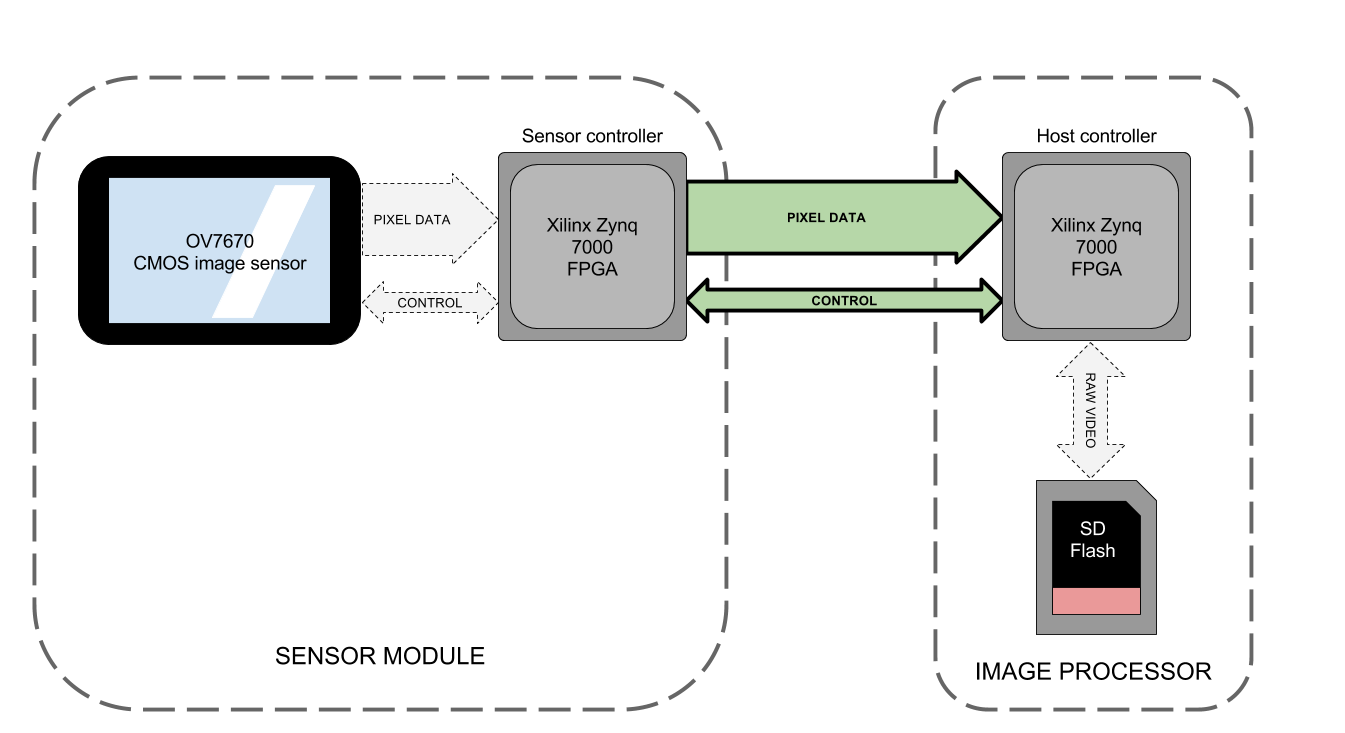
\includegraphics[width=1\textwidth]{./img/block_diagram_overview.png}
  \caption{Test system block diagram}
  \label{fig:block_diagram_overview}
\end{figure}

The system in Figure \ref{fig:block_diagram_overview} consists of an OmniVision OV7670 image sensor connected to a set of parallel inputs on a Xilinx Zynq 7000 \gls{fpga} acting as sensor controller. Pixel data is pulled from the sensor by the controller and placed into a \gls{ram} framebuffer where it can be retrieved by another part of the controller and transmitted across the interface. Optionally the controller can also generate a custom test pattern to be transmitted instead of the real sensor output for the purpose of system testing and benchmarking across a range of resolutions and framerates. These two components form the \textit{sensor module}, which is designed to be interchangeable with other sensor-controller pairs. The design of the interface highlighted in bold forms the main part of this project. 

On the master side of the interface is a second Zynq 7000 \gls{fpga} acting as the host controller. Pixel data going over the interface is received and decoded by the host before being stored in a framebuffer in \gls{ram}. The embedded ARM core inside the host forms the processing system, which takes each frame from \gls{ram} and serialises it into a RAW video stream in flash memory for playback on a computer. These components form the \textit{image processor}, which is capable of communicating with any connected \textit{sensor module}.

\subsection{Test system specification}

\begin{table}
  \centering
  \begin{tabular}{l | ll}
               & Minimum        & Maximum            \\
  \hline
  Resolution   & 320x240 (QVGA) & 2048x1080 (DCI 2K) \\
  Pixel depth  &                & 8-bit              \\
  Pixel format &                & Bayer RAW          \\
  Frame-rate   & 24p            & 60p                \\
  Throughput   &                & 1.2 Gbps          
  \end{tabular}
  \caption{Sensor interface specification}
  \label{table:interface_specification}
\end{table}

The specifications in Table \ref{table:interface_specification} were decided after surveying best-selling cameras across several markets, consisting of cinema cameras, \glspl{dslr} and computer-vision / industrial cameras.
  \chapter{Background}

This section presents a block diagram of a proof-of-concept system and introduces many of the concepts and motivations involved in understanding each block.

\section{System overview}

A block-diagram of the proof-of-concept system is illustrated in [Figure X]. The system is separated into two parts: the sensor module (consisting of image sensor and encoder FPGA) and the camera mainboard (with the approrpriate decoder FPGA).

[Insert system block diagram here]

\section{Field-Programmable Gate Arrays}

\subsection{Hardware Description Languages}
\subsection{Synthesis and Place-and-Route}

\section{CCD and CMOS sensor technologies}

The sensors themselves fall into one of two categories depending on technology used: \gls{ccd} and \gls{cmos}. While both use an array of photosites to collect charge from incident photons during exposure time, the readout and analogue-to-digital conversion process differs for each. During readout time, \glspl{ccd} sequentially shift the accumulated charges into horizontal and vertical readout registers where they are transferred to a chip-level output amplifier and analogue-to-digital converter to generate a binary bitstream. \gls{ccd} image sensors are capable of very low noise and high sensitivity due to the use optimised photosites; this made them a very popular choice for applications demanding high image quality.

Unlike \glspl{ccd}, which rely on a very specialised fabrication process, CMOS sensors can be manufactured using traditional \gls{cmos} processes, benefiting greatly from the associated economies of scale. \gls{aps}, the most common form of \gls{cmos} sensor, differ from \glspl{ccd} in that each photosite contains a dedicated amplifier, meaning that the light-induced voltages can be driven directly to the row and column decoders for digitisation. Because of the \gls{cmos} fabrication process, other camera functions can also be integrated onto the same chip, cutting both the cost and size of the device \cite{10_ge_2012}.  This level of integration, and the faster speeds of parallel readout processing have meant that \gls{cmos} sensors have seen a recent surge in popularity, and are forecast to account for 85\% of the total image sensor market in 2017 \cite{11_ic_insights_2013}.

\begin{figure}
  \centering
  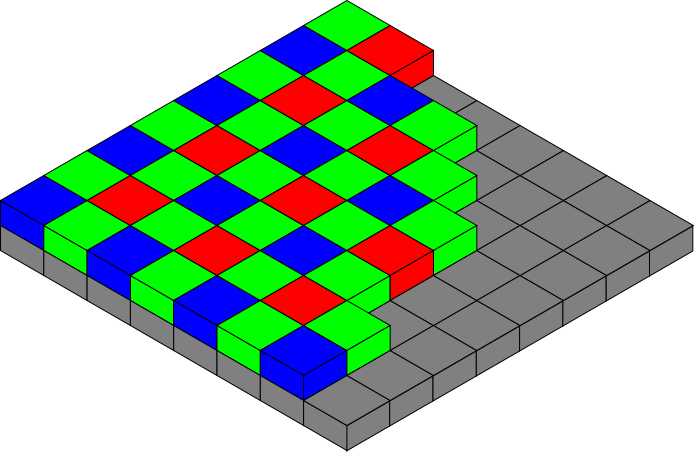
\includegraphics[width=1\textwidth]{./img/bayer_pattern.png}\par
Source: diagram by Cburnett, distributed under CC BY-SA 3.0
  \caption{Bayer filter}
  \label{fig:bayer_pattern}
\end{figure}

Photosites can only measure light intensity, not wavelength, producing greyscale images. By placing a coloured filter in front of each photosite, it is possible to only let light of a certain wavelength through \cite{12_eastman_kodak_company_1976}. Given the fixed pattern of the \gls{cfa}, it is possible to generate a full-colour image using a demosaicing algorithm, the simplest of which is bilinear interpolation, to calculate the red, green and blue intensities for each pixel \cite{13_malvar_he_cutler_2015}. One such \gls{cfa}, the Bayer filter, contains twice as many green elements as red and blue to mimic the physiology of the human eye, as illustrated in Figure \ref{fig:bayer_pattern}.
  \chapter{High-speed data transmission}

\section{Introduction}

While sensors can capture both still images and video, this project mainly concerns the latter due to its resource-intensive nature. A recent study found that 75\% of households in the United States had a high-definition television \cite{14_leichtman_research_group_2013}. The popularity of HD content makes it important to consider how bandwidth requirements increase with larger resolutions. An uncompressed 24-bit colour 1080p video at 24p has a bitrate of almost 1.2 Gbps, as calculated in Equation \ref{eq:hd_bandwidth}, well within the range where signal integrity becomes important.

\begin{equation}
  \begin{split}
    \mathbf{BW} &= (1920*1080) \, \mathrm{pixels} * 24  \, \mathrm{bpp} * 24 \, \mathrm{fps} \\
                &= 1.19  \, \mathrm{Gbps}
  \end{split}  
  \label{eq:hd_bandwidth}
\end{equation}

When transmitting a high-frequency signal between two devices, close attention must be paid to many aspects of the design to ensure that the signal integrity is preserved. The basic premise of signal integrity is covered here, however later sections will cover the issue in greater depth. With low-frequency signals, a wire or PCB trace can be modelled as an ideal circuit, without resistance, capacitance or inductance. As the frequency increases however, so-called transmission line effects are prominent and the \gls{ac} characteristics of the wire become very important. If there is a mismatch between the source, line and receiver impedances then the transmitted signal will not be fully absorbed at the load, resulting in any excess energy rebounding between source and receiver repeatedly until it has been fully absorbed. Due to superposition, the reflected waves will cause ringing and other signal integrity issues that reduce signal quality. If the issue is severe enough, the receiver cannot correctly interpret the signal and bit errors will occur. Parallel wires can also cause mutual inductance problems whereby the magnetic field generated by current travelling through one wire, will induce a current in the adjacent wire. Similarly, mutual capacitance is caused by the coupling of the two electric fields. These issues can be mitigated by taking care to ensure that impedance is properly controlled and \gls{pcb} traces are placed with care when designing circuits \cite{15_basic_principles_of_signal_integrity_2007}.

Table \ref{table:existing_protocols} shows a list of existing protocols / interfaces for transmitting image data.

\begin{table}
  \centering
  \begin{tabular}{llllll}
  Name      & Parent  & Family    & Bandwidth & Scheme  & Complexity \\
  \hline
  USB3 Vision   & USB 3   & USB       & 2.8 Gbps  & Serial  & High \\
  GigE Vision   & IP / UDP  & Ethernet    & 800 Mbps  & Serial  & Medium \\
  Camera Link   & N/A     & Camera Link   & 6.8 Gbps  & Serial  & Medium \\
  MIPI CSI-3  & M-PHY   & MIPI      & 23.2 Gbps & Serial  & Medium \\
  HDMI 2.0    & N/A     & HDMI      & 18 Gbps   & Serial  & Low / Medium
  \end{tabular}
  \caption{Existing protocols and interfaces for transmitting image data      \protect\cite{16_von_fintel_2013,17_arrowdevices.com_2014,18_hdmi.org}}.
  \label{table:existing_protocols}
\end{table}
  \chapter{Digital Video Interface}
\gls{dvi} is a video interface which surfaced in 1999. Designed by the \gls{ddwg} as a replacement for \gls{vga}, it was mainly used to display output from a computer's graphics adapter onto a monitor, although it did see some limited use in other entertainment equipment such as televisions and DVD players. Despite its age, the interface has more than enough bandwidth for 1080p RAW video and its relative simplicity makes it an attractive base for transferring image sensor data.

\section{Interface overview}

In \gls{dvi} nomenclature, a \gls{dvi} link is comprised of an input and output video stream, and the corresponding \gls{tmds} circuitry which is used to transmit the video from one side of a link to the other. Figure \ref{fig:dvi_link_overview} illustrates a typical single-link, consisting of a transmitter / receiver pair joined by four serial \gls{tmds} channels. In the standard RGB operating mode, the three colour components (red, green and blue) are separated and transmitted one per channel, with the remaining channel being used to carry the pixel clock. In addition to pixel data, each channel also has two bits for control signals. On the blue channel (channel 0), the control lines are used to carry the horizontal and vertical synchronisation signals needed for data recovery at the receiver. All other control lines are reserved for future use.

\begin{figure}
  \centering
  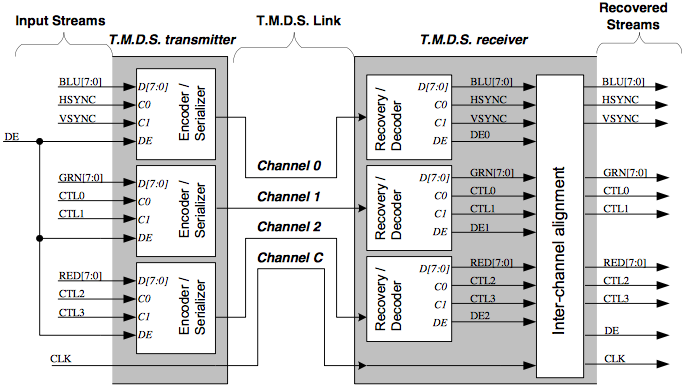
\includegraphics[width=1\textwidth]{./img/dvi_link_overview.png}\par
Source: DVI 1.0 Specification
  \caption{Single \gls{dvi} link in RGB mode.}
  \label{fig:dvi_link_overview}
\end{figure}

\subsection{Video format and timing}

Unlike other modern digital video interfaces, \gls{dvi} does not packetise its data for transmission. Instead, it uses a legacy raster scan technique which was originally intended to drive the electron gun inside a \gls{crt} display. While raster scanning is redundant for digital displays, \gls{dvi} opts for this technique in order to ensure backwards compatibility with the \gls{vga} interface, which was originally designed for use with analogue \gls{crt} displays.

\begin{figure}
  \centering
  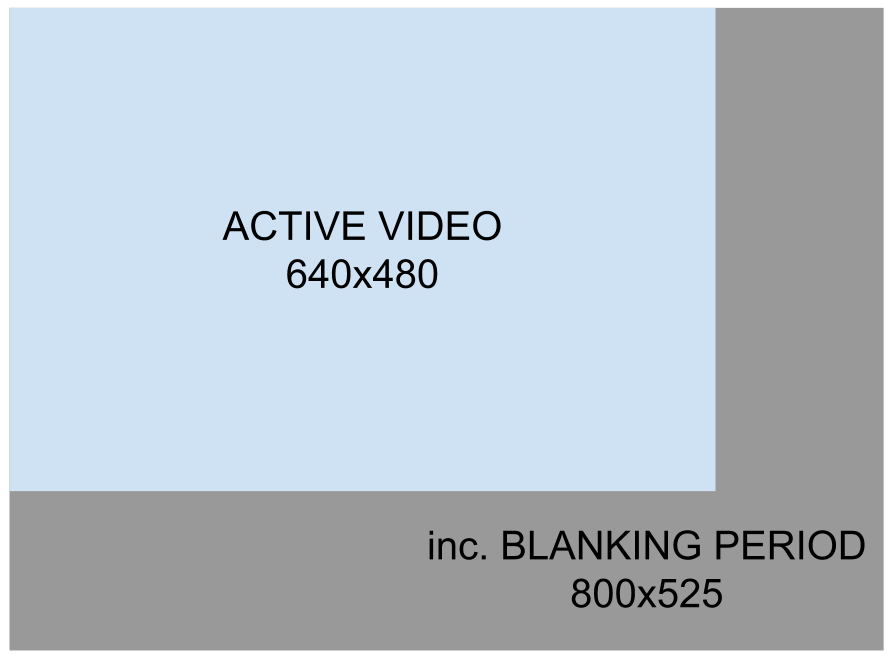
\includegraphics[width=1\textwidth]{./img/raster_scan.png}
  \caption{Illustration of visible pixels and blanking periods.}
  \label{fig:raster_scan}
\end{figure}

\begin{figure}
  \centering
  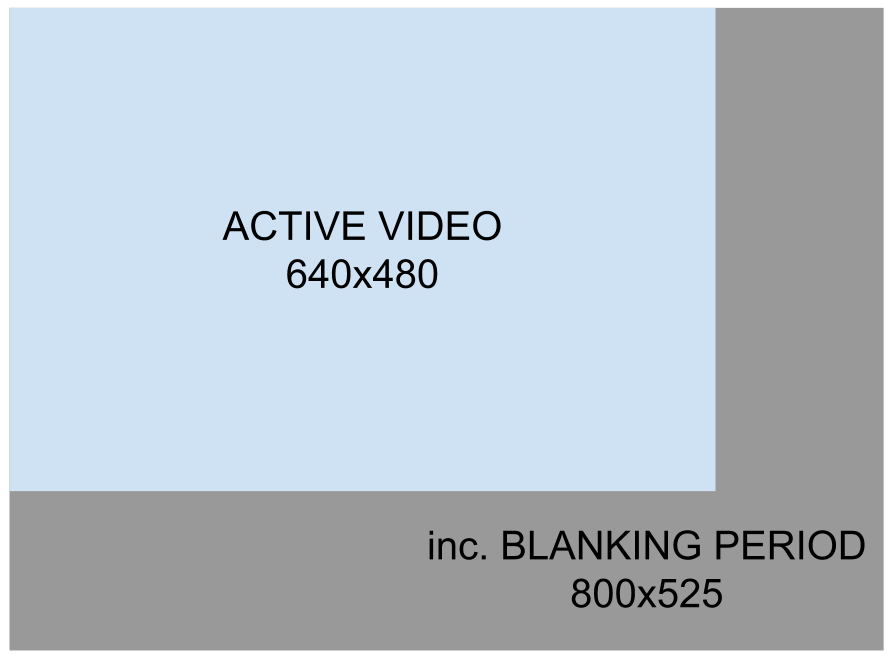
\includegraphics[width=1\textwidth]{./img/raster_scan.png}
  \caption{Video timing synchronisation signals used to mark end of line (HSYNC) and end of frame (VSYNC).}
  \label{fig:video_timing_signals}
\end{figure}

Figures \ref{fig:raster_scan} illustrate the raster scan video technique. If this image was displayed on a monitor, only the blue 'active video' part would be visible, while the grey 'blanking period' extends beyond the display and thus is not drawn, rather it is used to carry the timing signals in Figure \ref{fig:video_timing_signals}. In an analogue monitor these signals would have been used to position the electron beam, however in modern digital displays the HSYNC (end of line) and VSYNC (end of frame) signals are used to detect the video resolution. A list of common video timings can be found in Table.\marginpar{Need to add a table for this}. Single-link \gls{dvi} requires all devices to support a colour-depth of 24-bits per pixel. Unlike \gls{hdmi}, which supports both RGB and YUV data formats, \gls{dvi} only supports RGB.

\subsection{Physical layer}

\gls{dvi} utilises \gls{tmds} in order to reduce \gls{emi}, improve noise immunity and increase skew tolerance for driving data through longer cables. Although the proof-of-concept presented here utilises a cable to link the sensor module and image processor together, noise immunity and skew tolerance are not particularly useful as a real commercial system would use a board-to-board connector to mate the two systems directly together. As mentioned in the overview, a \gls{tmds} link consists of three completely separate data channels and a clock channel. Because of the colour component separation, all three channels are functionally identical and can operate independently of each other; though the clock channel is required for synchronisation.

Like most other high-speed serial interfaces, \gls{tmds} utilises a line coding scheme in order to ensure low \gls{emi}, better noise immunity and skew tolerance. The function of the \gls{tmds} encoder is to take the parallel 8-bit pixel value and 2-bit control data, and convert them into a 10-bit character which may utilise these attributes. Figure \ref{fig:dvi_link_overview} illustrates how the red, green and blue channels are fed into the corresponding encoders (all of which are functionally identical) to produce three serial streams of 10-bit \gls{tmds} characters. Only pixel data or control data may be transmitted at any one time, and so an additional data input signal is required to determine whether the 10-bit \gls{tmds} character is produced from the pixel data (\texttt{DE = 1}) or the control data (\texttt{DE = 0}). 

In order to reduce the number of transitions (and thus the \gls{emi}), the encoder uses a special algorithm for pixel data which produces characters with no more than five transitions, however control data characters use a different algorithm which can produce over seven transitions, though the relatively short duration of the blanking period ensures this is not an issue. Despite all three channels being referenced to the same pixel clock, there is a high chance of the three channels being out of phase at the receiver as a result of trace-length mismatches and various other factors which introduce signal skewing. For the receiver to function correctly, all input channels need to be phase-aligned. To aid this, the \gls{tmds} encoder produces long runs of similar characters which can be easily detected by the receiver in order to mark character boundaries and align the channels.

\gls{tmds} is a serial protocol, and thus the 10-bit output characters from the encoder are serialised and transmitted alongside a \gls{tmds} reference clock. While increasing the maximum bandwidth, serial transition also reduces cost and complexity, allowing a minimal \gls{dvi} interface to be implemented using only four wires. Unlike some high-speed serial interfaces, the clock does not need to be recovered from the data as it is transmitted alongside it. Every clock cycle the \gls{tmds} transmitter outputs a 10-bit character.

\subsection{DDC and EDID}

Alongside the \gls{tmds} signals, \gls{dvi} also includes an I\textsuperscript{2}C-based \gls{ddc} interface for communication between the graphics host and display device. While variants of \gls{ddc} exist which allow for complex heirarchies of devices and bidirectional communication, \gls{dvi} only requires DDC2B to be implemented.

The DDC2B interface allows for a graphics host and display device to be connected in a master / slave configuration, with the graphics host always designated as bus master. As the interface is based on the I\textsuperscript{2}C protocol, each slave must be assigned an address so that other devices can talk to it. In DDC2B the slave is assigned address \texttt{0xA0} (\texttt{0xA0} for writes, \texttt{0xA1} for reads). Figure \ref{fig:i2c_bus} shows a simple master / slave configuration.

\begin{figure}
  \centering
  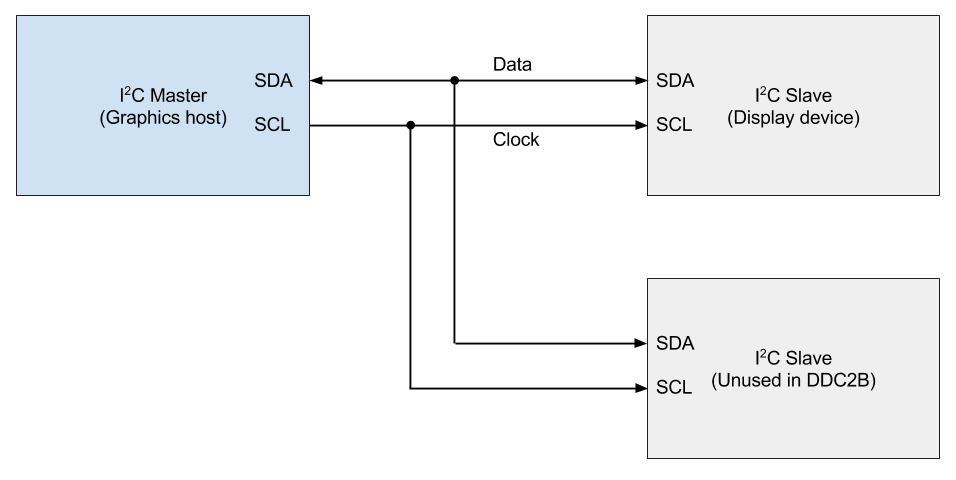
\includegraphics[width=1\textwidth]{./img/i2c_bus.png}
  \caption{A typical I\textsuperscript{2}C master / slave configuration. DDC2B specifies a single master (graphics host) and a single slave (display device).}
  \label{fig:i2c_bus}
\end{figure}

I\textsuperscript{2}C requires only two nets, regardless of the number of master and slave devices, thus it is a very simple and cost effective protocol. I\textsuperscript{2}C messages are one of two types: address frames and data frames. When the master wants to read data data from a slave, it sends out a frame with the address of the slave followed by a data frame containing any additional information (such as a specific register to read), the slave then responds with a data frame containing the requested data.

\gls{edid} is a standardised data structure which may be used by a display device to describe various capabilities such as supported resolutions and colour formats. Typically the \gls{edid} data is stored on an I\textsuperscript{2}C-connected \gls{eeprom} chip inside the display device, so that the graphics host may query the display's capabilities using the \gls{ddc} and set the output format accordingly. (http://read.pudn.com/downloads110/ebook/456020/E-EDID%20Standard.pdf).

\begin{table}
    \begin{tabular}{ll}
    Byte offset & Field                       \\
    0x00        & Header information          \\
    0x14        & Basic display parameters    \\
    0x19        & Chromaticity coordinates    \\
    0x23        & Established timing bitmap   \\
    0x26        & Standard timing information \\
    \end{tabular}
    \caption{Basic fields \gls{edid} v1.3 for storing monitor capabilities.}
    \label{table:basic_edid_fields}
\end{table}

\section{Required additions for image sensors}

While \gls{dvi} provides a suitable transport for the video stream, it lacks various other features which would be required for a standardised image sensor interface. Chief among these is the means with which to synchronise devices to the electronic shutter on the image sensor. While mirrorless cameras are gaining popularity, cameras with mechanical shutters are still very common. Mechanical shutters come in many different varieties, but they all require very tight syncrhonisation with the electronic shutter in the sensor to light is captured correctly (the former controls when the light hits the sensor, while the latter controls when each photosite on the sensor starts and stops capturing the light). To ensure the image is exposed correctly it is important to synchronise all of the components downstream from image sensor which affect exposure. An example of poor synchronisation between these components can produce effects like those seen in Figure \ref{fig:flash_unsync}. To prevent this from happening, the image sensor needs to be able to signal exactly when it is about to start exposure so that any downstream components may synchronise themselves accordingly.

\begin{figure}
  \centering
  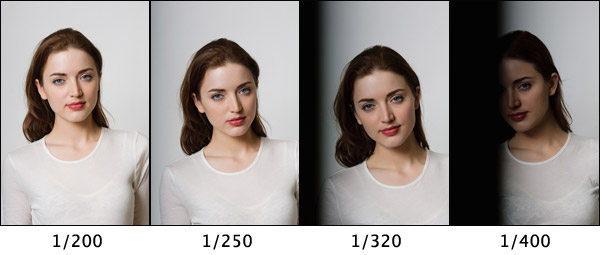
\includegraphics[width=1\textwidth]{./img/flash_unsync.jpg}\par
Source: http://neilvn.com/tangents/auto-fp-flash-setting-nikon-d300s-d700/ 
  \caption{Lack of synchronization between mechanical shutter and flash prevent parts of the image sensor from being exposed.}
  \label{fig:flash_unsync}
\end{figure}

As image sensor modules must be interchangeable, it is essential that the camera body is able to query each sensor's capabilities to ensure compatibility and sufficient performance in the parts of the design which are dependant on image format. Key capabilities are image resolution, video framerate, electronic shutter type (rolling or global) and bit depth. Additionally, image sensors use several different types of \glsp{cfa}, and so to be able to de-mosaic the image (interpolate RGB colour values), knowledge of the Bayer pattern used is required. For the image processor to be able to display colour images on the viewscreen it needs to be able to query the Bayer pattern type from the image sensor. 
 
Leading on from this, high-performance camera systems capture and store the raw greyscale output from the image sensor (hence the RAW format), avoiding in-camera image processing as much possible to ensure lossless image capture. \gls{dvi} only supports the RGB format and so needs extending to be able to transport high bit-depth RAW format data.
 
The technical details of each of these additions is described in the implementation part of this report.

\marginpar{Don't forget to reference this whole section to the DVI spec - once per paragraph}
  \newcommand{\ov7670_capture}{\texttt{ov7670\_capture}}

\chapter{Design and Implementation}

\section{OV7670 sensor controller}
\subsection{Overview}
To prove that the interface was suitable for image sensors a 640 x 480 OV7670 CMOS sensor was used to capture real-time image data... The Omnivision OV7670 is a small, low-cost CMOS sensor originally design for use in mobile phones which has seen popularity in the hobbyist electronics community due to its availability and ease of use. These factors, along with the wealth of documentation available contributed to its inclusion in this proof-of-concept system. As mobile phone at the time lacked the power to do image processing themselves, the OV7670 contains built-in hardware for image enhancements such as de-bayering, lens correction and noise removal, making it surprisingly complex. The OV7670 was included solely to demonstrate the effectiveness of the interface in a real camera system, thus these features are not used.

\begin{figure}
  \centering
  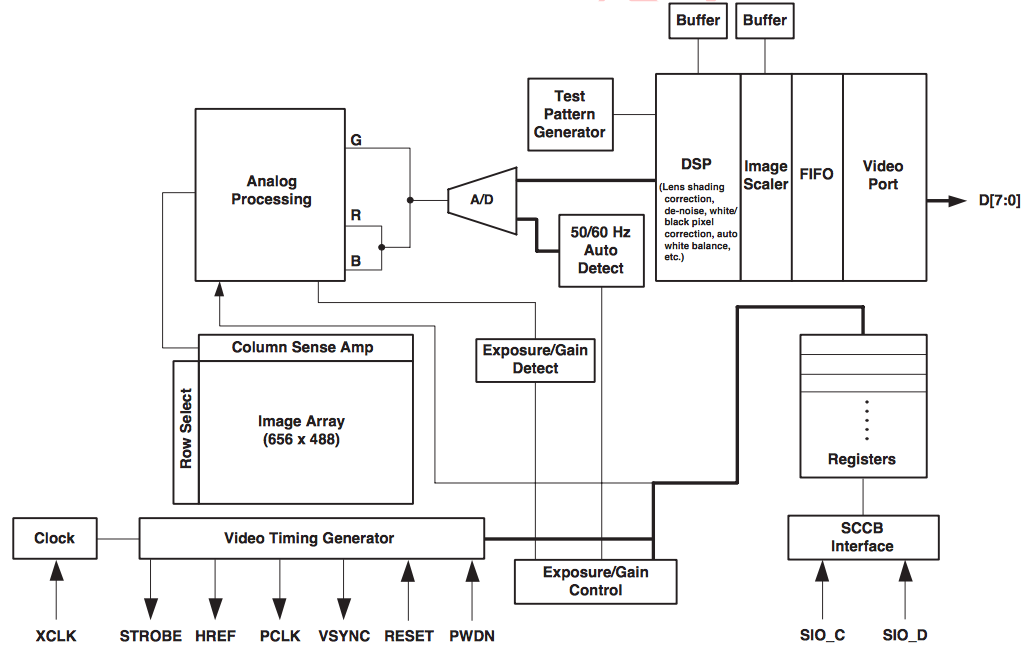
\includegraphics[width=1\textwidth]{./img/ov7670_block_diagram.png}\par
Source: Omnivision OV7670/OV7171 1.0 Specification
  \caption{Functional block diagram of Omnivision's OV7670 CMOS image sensor.}
  \label{fig:ov7670_block_diagram}
\end{figure}

Figure \ref{fig:ov7670_block_diagram} outlines the key functional blocks inside the OV7670. Light is captured by a 656 x 488 array over a specific duration of exposure. From here it is read out one row at a time into the analogue processing block which performs white-balance adjustments and amplifies the signal to increase sensitivity. From here it is digitised and fed into an image processing block for lens correction, de-noising and various other enhancements. Image scaling is also performed, before it is piped into a \gls{fifo} buffer ready for output on the 8-bit parallel video interface. The pixel size depends on the pixel format used: the RAW format only uses 8 bits and a single pixel can be output each clock cycle, while the RGB 4:2:2 and YUV 4:2:2 formats require 16 bits, thus taking two clock cycles per pixel. To construct a complete frame from the output pixels we require some additional information provided by the video timing generator in the form of vertical and horizontal synchronisation signals. The synchronisation signals in Figure \ref{fig:ov7670_timing} can be used to keep track of which the starting point of the each frame, and signals whether or not the pixel data on \texttt{D} can be sampled. 

\begin{figure}
  \centering
  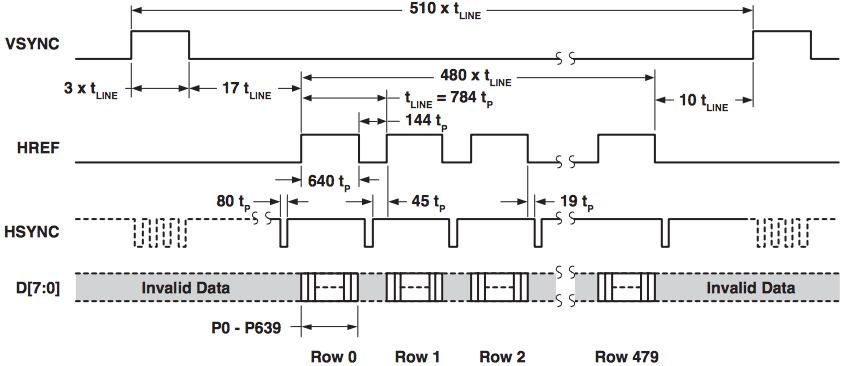
\includegraphics[width=1\textwidth]{./img/ov7670_timing.png}\par
Source: Omnivision OV7670/OV7171 1.0 Specification
  \caption{OV7670 timing diagram. The \texttt{VSYNC} signal pulses shortly before the start of each frame. \texttt{HREF} is high to indicate the data on output \texttt{D} is valid.}
  \label{fig:ov7670_timing}
\end{figure}

\subsection{\texttt{ov7670\_controller} module}
The OV7670 contains a set of internal registers to configure all aspects of its operation. In order to set the output format to 640 x 480 RAW the correct registers must be set using the \gls{sccb} protocol --- a direct clone of I\textsuperscript{2}C, renamed for licensing / IP reasons. As we are only interested in writing to specific registers there is no need to implement bidirectional I\textsuperscript{2}C communication. To drive the \gls{sccb} interface the \texttt{ov7670\_controller} module utilises I\textsuperscript{2}C code written by Mike Fields (http://hamsterworks.co.nz/mediawiki/index.php/Zedboard_OV7670). Table \ref{table:ov7670_register_settings} lists the register settings used to configure the OV7670 for 640 x 480 RAW output at 30 \gls{fps}. On powerup, the \texttt{ov7670\_controller} module performs the following actions for each register it configures:

\begin{enumerate}
    \item Pull \texttt{SDA} low to signal master is about to send
    \item Send 8-bit address frame with value 0x42
        \begin{itemize}
            \item \texttt{Bits 7--1}: OV7670 I\textsuperscript{2}C slave address \texttt{0x21}
            \item \texttt{Bit 0}    : \texttt{R/W = 0} to write to register) 
        \end{itemize}
    \item Pause to allow OV7670 to acknowledge address frame
    \item Send 8-bit data frame with address of configuration register
    \item Pause to allow OV7670 to acknowledge data frame
    \item Send a second data frame with value to write to configuration register
    \item Pause to allow OV7670 to acknowledge data frame
\end{enumerate}

The \texttt{ov7670\_controller} module contains a 'dumb' I\textsuperscript{2}C controller --- it ignores all responses from the slave and stops as soon as it has finished configuring the OV7670 registers. For the sake of simplicity, the register configuration can be re-triggered by asserting the reset signal. Not implementing intelligence to deal with frame retransmits due to errors simplifies the design significantly, while still allowing the user to manually re-trigger register configuration if anything does go wrong. Once the configuration has been written the \texttt{ov7670\_controller} module asserts the \texttt{start\_capture} signal to notify the \texttt{ov7670\_capture} module that the OV7670 is initialised and properly configured.

\begin{table}
    \begin{tabular}{llll}
    Register            & Address   & Value     & Description                       \\
    COM7                & 0x12      & 0x80      & Reset all registers to defaults   \\
    CLKRC               & 0x11      & 0x01      & Input clock prescaler divide-by-four, disable PCLK doubling (PCLK will be \(f_internal / 2\)) \\
    DBLV                & 0x6B      & 0x7A      & Input clock PLL x4                \\
    COM7                & 0x12      & 0x01      & Output format 640 x 480 Bayer RAW \\
    COM3                & 0x0C      & 0x00      & Disable output scaling            \\
    COM14               & 0x3E      & 0x00      & No PCLK scaling                   \\
    SCALING_XSC         & 0x70      & 0x3A      & Magical horizontal scale factor   \\
    SCAKING_YSC         & 0x71      & 0x35      & Magical vertical scale factor     \\
    SCALING_DCWCTR      & 0x72      & 0x11      & Downsample by 2           \\
    SCALING_PCLK_DIV    & 0x73      & 0xF0      & No PCLK scaling           \\
    SCALING_PCLK_DELAY  & 0xA2      & 0x02      & Scaling output delay 2    \\
    \end{tabular}
    \caption{(Based on values in OV7670 datasheet and implementation guide)}
    \label{table:ov7670_register_settings}
\end{table}

\subsection{\texttt{ov7670\_capture} module}
\marginpar{Code snippets required!}
Given that the purpose of a standardised image sensor interface is to provide video data in a format which can be paired with any image sensor device, it stands to reason that the data must be converted to a different format at some point. The task of the \ov7670_capture module is to capture pixels from the OV7670's parallel video interface and pass them on to the \texttt{i\_buf\_controller} module detailed in Section \ref{sec:framebuffer_dma} for storage in the framebuffer where they are processed by the DVI encoder. Originally the \ov7670_capture module had direct control over the memory, however this functionality was moved to the \texttt{i\_buf\_controller} module, reducing the \ov7670_capture to a passthrough or level conversion device.

To transfer frames between different blocks inside the \gls{fpga}, uses the standard VESA video interface: a pixel clock to signal when a new pixel is available, parallel data for pixels, horizontal sync for signalling end-of-line, vertical sync for signalling end-of-frame, and additionally a data valid signal which marks exactly when the active video period begins---greatly simplifying the design. Without this signal a timing recovery block would be needed to measure the frequency of \texttt{vsync} and \texttt{hsync} pulses to determine the resolution of the video and thus where the active video period begins and ends.

The OV7670's video interface is very similar, however some signals are lacking and others function differently as summarised in Table \ref{table:ov7670_video_interface}. 

\begin{table}
  \begin{tabular}{lll}
  OV7670 signal   & VESA equivalent & Description                                           \\
  d[7:0]          & d[7:0]          & Pixel data remains the same                           \\
  vsync           & vsync           & OV7670 vsync is active-high, VESA vsync is active-low \\
  href            & vde             & href is active-low, vde is active-high                \\
  N/A             & hsync           & OV7670 lacks a href signal
  \end{tabular}
  \caption{The OV7670 video interface is very similar to the VESA interface, however minor signal conversions are required.}
  \label{table:ov7670_video_interface}
\end{table}

\marginpar{Write about shutter_sync generation}


\marginpar{NEEDS A PICTURE OF OV7670 MODULE!}

\section{Framebuffer DMA processor}
\label{sec:framebuffer_dma}

A framebuffer is a portion of memory which holds the current frame, allowing the hardware blocks either side to act in complete isolation. Both sides of the link use framebuffers, though their purpose differs. On the receiver side the framebuffer stores each frame before it is written to flash storage. Firmware inside the Zynq \gls{ps} \marginpar{Explain the Zynq PS} can draw to the frame in real-time, adding helpful indicators such as the currently connected sensor module and gridlines to aid the photographer's composition process. On the transmitter side the framebuffer serves a different purpose. A critical flaw in the design of the \gls{dvi} receiver causes the link to break if the incoming pixel clock is less than \SI{40}{\mega\hertz} --- a potential issue because the OV7670's pixel clock is only \SI{12}{\mega\hertz}. To mitigate this, the transmitter sends out duplicate frames, thus bringing the pixel clock up into the region required for correct operation.

The space required to store frames is a direct function of the image resolution. As the OV7670 outputs frames in 640 x 480 resolution, a \SI{307.2}{\kilo\bytes} framebuffer is required. While \glsp{fpga} usually contain a small amount of internal block RAM, there is insufficient space for storing an entire frame. Though its access is significantly more complicated, the Zynq-7000 includes a hard DDR controller which can be utilised to store the frames in external DDR3 memory instead --- the Zybo development board contains \SI{512}{\mega\bytes} of RAM, which is more than sufficient for storing a single frame. Due to the internal architecture of the Zynq-7000, the \

\marginpar{Diagram of internal Zynq arch - access to DDR}

\marginpar{Diagram of OV7670 -> framebuffer -> DVI isolation, and DVI -> framebuffer -> SD / screen}



\section{DVI encoder}

\marginpar{Include formula for exact throughput, and pixel clocks used for OV7670}

\section{DVI decoder}
\section{EDID subsystem}
\section{Exposure sync subsystem}
\section{Flash storage manager}
\section{Viewscreen controller}
\section{Test pattern generator}
\section{Sequence detector}

  \chapter{Testing and analysis}
    \section{OV7670 image capture}
    \section{Continued operation}
    - Record device temperature
    - Warmup period?
    \section{Critical path}
    \section{Maximum throughput}
  
  \chapter{Conclusion}

  \marginpar{NO CAMERA CONTROL (start record... - master -> slave control channel?)!}

  \marginpar{NO PICTURES OF CAMERA!}

  \marginpar{NO PICTURES FROM CAMERA!}

  \chapter{Further work}

  \marginpar{NO CAMERA CONTROL!}

  \marginpar{NO CAMERA PICTURES!}

  \bibliographystyle{IEEEtranN}
\bibliography{bibliography_broken}
  \printglossary[type=\acronymtype]

\end{document}